\chapter{Results}\label{results}

\todo[inline]{Revision 3}

In the previous chapter the research background and methodology adopted during the work were presented. This chapter summarises the papers that added to the research contributions.

\section{Papers}\label{papers}

The research work has been published in two journal papers and four conference papers, one paper is currently ready for submission. In this section, papers that presents the results of this thesis are summarised. Each summary includes: 
\begin{itemize}
	\itemsep1pt\parskip0pt\parsep0pt 
	\item Title 
	\item Authors and roles in the paper 
	\item Abstract of the paper
	\item Where the paper was published 
	\item A short description of the results 
	\item The paper's relation to research questions 
\end{itemize}

Papers are reprinted in full in Appendix \ref{papers} of the thesis.

In addition to the papers presented in this section this PhD work has produced fourteen peer-reviewed secondary papers presented in conferences and workshops which are omitted in this section. Those works present incremental achievements in research that led to the results presented here. A brief description of secondary papers is included in Appendix \ref{secondary-papers}

\section[CroMAR: Mobile Augmented Reality for Supporting Reflection on Crowd Management]{Paper 1} \label{paper-1}

\emph{Title}: CroMAR: Mobile Augmented Reality for Supporting Reflection on Crowd Management

\emph{Authors}: Simone Mora, Alessandro Boron and Monica Divitini

\emph{Authors' contributions}: Mora led the research and the paper writing. He was actively involved in design, development, and evaluation of the system. Boron developed part of the described prototype and contributed to the paper with the description of the technical implementation. Divitini provided~general~supervision for the research and the paper writing. 
\begin{quote}
	\emph{Abstract:} This paper discusses the usage of Mobile Augmented Reality (MAR) to support reflection on past events, using reflection on crowd management as scenario. Computer based support to reflection generally relies on the visualization of information connected to the experience one is reflecting upon. Different metaphors have been adopted to support easy access to relevant information within the reflection process, e.g., timelines and word clouds. In this context, MAR represents an interesting alternative because it can be used to promote reflection in the specific location of the event by augmenting it with relevant information. In this way, the authors can expect the reflection process to be grounded in a context that helps to make sense of the information and reflect on alternative paths of action. The paper presents the scenario of usage, together with the design, development, and evaluation of the prototype, CroMAR. Based on this experience, the authors identify challenges connected to the usage of Mobile Augmented Reality in terms of support for reflection, interaction, and design methodology. 
\end{quote}

\emph{Published in}: International Journal of Mobile Human Computer Interaction (IJMHCI), 2012

\emph{Description}: This paper investigates the adoption of Mobile Augmented Reality (MAR for short) to support debriefing of work practices that rely on management of resources in space. To date, it is the first time that MAR is used for such purpose. Crowd management, an activity typically performed by civil protection organisations during large public events, is scrutinised to investigate the use of augmented reality to support (collaborative) reflection processes after the event is concluded. Crowd management is a critical activity both for crisis preparedness and during crisis management.

CroMAR, an iPad app designed by the authors, demonstrated the use of MAR for reflection. The system developed focuses on supporting navigation of reflection-useful information along the time and space dimension. Visualisation of information is provided in-situ, in a physical context that helps making sense of the information and reflect on alternative paths of actions. Also, the system provides support in involving others in the reflection process and in sharing of its outcome.

The proposed design has been implemented in a working prototype of an iPad app (Figure \ref{fig:cromar-prototype}), with focus on modularity and extensibility. The prototype has been evaluated in a focus group with experts. The study highlights challenges in supporting reflective learning with MAR tools, with focus on user experience. First the research requires a better understanding of the conditions that makes MAR a better approach compared to other visualisation approaches (e.g.~maps, timelines). Second, it claims the need for providing scaffolding mechanisms to the reflection process; to make sure that relevant information for a given session is explored. Acknowledged by experts that the physical exploration of space provide scaffolding for exploration of information, it is necessary to study when it actually promotes reflection. 

\begin{figure}
	[tbh] \centering 
	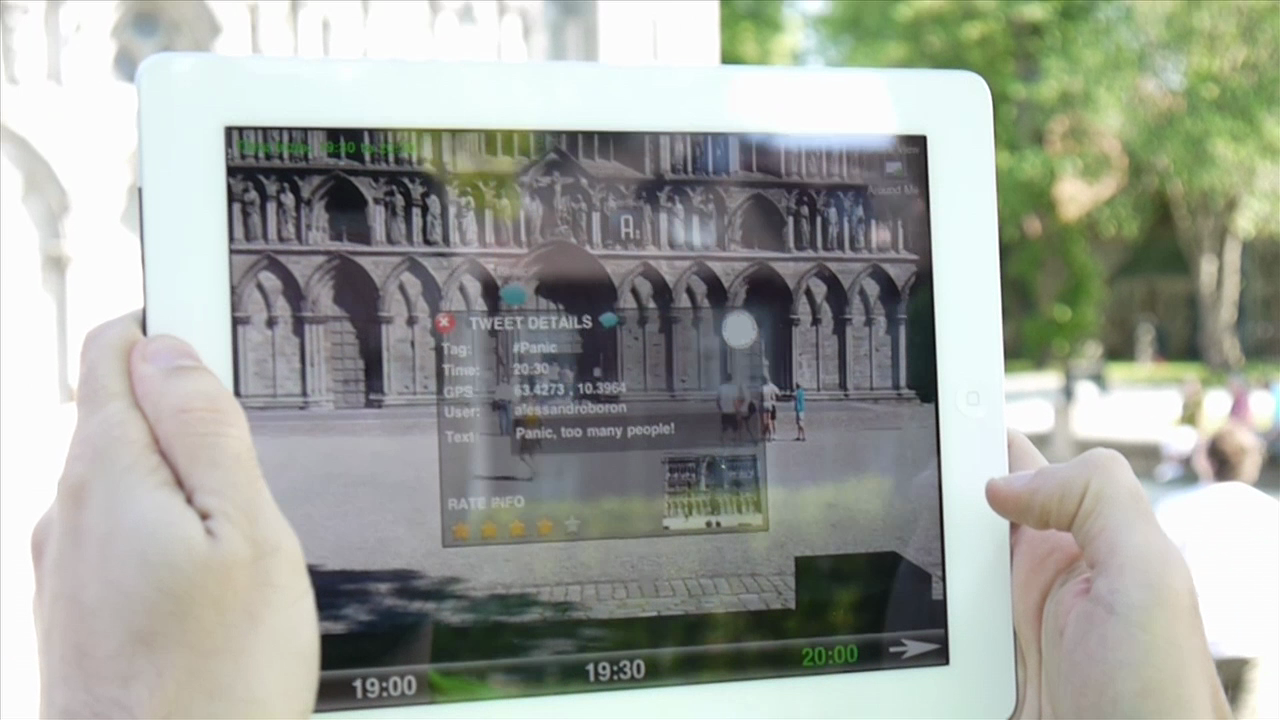
\includegraphics[width=1 
	\textwidth]{cromar_1stproto} \caption{CroMAR early prototype} \label{fig:cromar-prototype} 
\end{figure}

During our evaluation, the overall user experience with the prototype was hampered by lack of functionalities and lack of suitable hardware platforms. The experience is disrupted by the lack of tools for filtering the data visualised, to remove redundant information and prioritise the important ones. On the other side, the choice of iPads 2 has limitation due to device weight and size which can only be comfortably hold by the user for a few minutes.

The results from this paper have fed new design iterations for CroMAR. The design of new functionalities has followed more closely the guidelines provided by the CSRL model that was being developed at the time. Meanwhile lighter and smaller version of the iPad came to the market which allowed an extended use for our system. A new prototype of CroMAR and its closer mapping to the CSRL model is described in P2.

\emph{Relation to the research questions: } The paper started the investigation of RQ2, ``\RQii'' 

\section[Supporting Debriefing with Sensor Data: A Reflective Approach to Crisis Training]{Paper 2}\label{paper-2}

\emph{Title:} Supporting Debriefing with Sensor Data: A Reflective Approach to Crisis Training

\emph{Authors:} Simone Mora and Monica Divitini

\emph{Authors' contributions:} Mora led the research and the paper writing. He also led the design of the presented technology and directly implemented or supervised the implementation of the prototypes. Both authors attended the evaluation studies. Divitini provided general supervision for the research and the paper writing.

\begin{quote}
	\emph{Abstract:} In this paper we present our exploration into the use of sensor data to promote debriefing after training events simulating work experiences. In this way we address one of the core challenges of crisis training, namely the difficulty to exploit the full potential of training events, e.g.~during drills. The paper is theoretically grounded in the theory of reflective learning. The theoretical understanding is used for informing the design of WATCHiT, a wearable device for collecting sensor data during an event, and two applications for promoting debriefing in two different scenarios, CroMAR and Procedure Trainer. CroMAR supports disaster managers during in-situ debriefing after large events, while Procedure Trainer supports a team in reflecting after the simulation of a medical emergency procedure. The evaluation of the two applications shows that sensor data can be successfully used to support debriefing in both scenarios. Based on our experience, we draw lessons learned for the design of systems supporting debriefing in training events. 
\end{quote}

\emph{Published in:} Proceedings of Information Systems for Crisis Response and Management in Mediterranean Countries (ISCRAM-MED), 2014

\emph{Description:} The paper focuses on supporting with sensor data the activity of debriefing after training events simulating work experiences (e.g.~physical simulations). 

To increase the efficacy of debriefing, and thus their impact on crisis preparedness, it is important to exploit the full potential of training events, which are costly to organise. There are different forms of debriefing, all complex activities that may vary in terms of details and people involved according with the emergency scenario workers have been training on. Debriefing is made difficult by the highly distributed nature of the work, the co-existence of different partial experiences and lack of data to complement human memories of the event. The paper addresses those challenges presenting an ecology of three applications of sensing-based technology to assist different debriefing scenarios. Two applications: \emph{CroMAR} and \emph{WATCHiT} have been described in P1 and P3 and are here presented in the last stage of their evolution. Trainer, introduced in this paper, is an smartphone application to support a quick reflection session on the implementation of protocols (e.g.~medical procedures) that can be done by the worker herself or in a team. In this work technology mapping with the CSRL model is made explicit.

The three applications presented have been evaluated during simulated crisis work events. Building on evaluation results, the paper presets lessons learnt about the use of sensor data for supporting debriefing and the design of systems to support reflection during debriefing. 

\emph{First} it is acknowledged that sensor data has to be complemented by qualitative information in order to set the right focus for reflection and avoid over-sighting qualitative, yet critical aspects of the work that cannot be captured with quantitative methods.

\emph{Second} it suggests the use of \emph{visualisation} and \emph{storytelling} as mechanisms to promote sense-making processes for turning data into useful learning contents. Visualisation helps understanding the data by \emph{re-creating} a context that help spotting discrepancies with other sources and, in turn, to trigger reflection. For this goal it is important that systems allow to compare data against a baseline or other sources. Storytelling happens when a visualisation need to be interpreted and explained both to the self and to others, connecting data to the human memory of the event; as it was observed during evaluations. Also, how to motivate the user in capturing data needed for visualisation and storytelling is still an open challenge.

\emph{Third}, the proposed technologies aim at bringing debriefings out of the traditional office setting but not as substitutes, rather to complement the current practices by creating smooth transitions among different debriefing (and thus reflection) cycles. These propositions will guide future research to leverage sensor data in debriefings.

\emph{Relation to the research questions:} The paper covers aspects of RQ1 ``\RQi'' and RQ2, ``\RQi''

\section[WATCHiT: a modular and wearable tool for data collection in crisis management and training]{Paper 3}\label{paper-3}

\emph{Title:} WATCHiT: a modular and wearable tool for data collection in crisis management and training

\emph{Authors:} Simone Mora and Monica Divitini

\emph{Authors' contributions:} Mora led the research and the paper writing. He also presented the paper at the conference. Mora directly implemented or supervised the implementation of the prototypes. He also conducted the field studies and evaluations. Divitini provided general supervision for the research and the paper writing.

\emph{Published in:} Proceedings of the European Conference in Ambient Intelligence (AMI), 2014 

\begin{quote}
\emph{Abstract:} We present WATCHiT, a prototype of sensor-augmented wristband computer for data collection during crisis response work. During crises, information about the environment (e.g.~to map the territory) and the rescuers (e.g.~for assessment of workers' condition) offers help to support coordination of work, post-emergency debriefing and to build realistic training scenarios. Being each crisis nearly unique it is important to collect data from every single occurrence, yet it is difficult to foresee the type of data and context information that is relevant to capture. WATCHiT features: (1) wearable sensors, (2) easy customisation of the type of information sensed, including both quantitative and qualitative data; (3) an intuitive, distraction-free user interface for controlling the data capturing procedure. Our design process has been driven by user studies during training events characterised by a high degree of realism; our prototype has been successfully evaluated with experts against technology acceptance. 
\end{quote}

\emph{Description:} This paper presents the design research that led the development of WATCHiT, a wearable computer for data collection in-action during crisis response work (Figure \ref{fig:watchit-prototypes}). The design research has followed four steps. Field studies conducted by the authors have produced seven challenges for the design of technology tools to support data collection during real or simulated crisis. Those design opportunities are summarised in Table \ref{tab:design-challenges}. User studies were performed during physical simulation of crisis work. Simulations were organised to provide a high degree of realism, involving dozens of agents; and recreating working conditions as close as possible to real crises.

\begin{table}
	[tbh] \centering \caption{Design challenges for data collection tools in crisis work} \label{tab:design-challenges} 
	\begin{tabular}
		{@{}p{0.05\linewidth}p{0.25\linewidth}p{0.60\linewidth}@{}} \toprule & Challenge & Description \\
		\midrule DC1 & Mobility of work and sensing & It is important to complement data from sensors embedded in the environment with mobile ones. The degree of mobility and thus granularity of data is important. Fine granular data is achieved with sensors worn by first responders. \\
		DC2 & Different crises, different relevant data & Being each crisis almost unique, it is difficult to define which data might be relevant to capture based on generic typologies of crises. \\
		DC3 & Different types of data & Different types of information are relevant to be captured. Including information for assessment of the worker’s safety, for mapping the territory and the work and Information related to the rescued people (e.g. type of injures). \\
		DC4 & Sensor data and user-submitted data & Workers might however provide critical qualitative data that cannot be measured with sensors to complement quantitative ones. \\
		DC5 & Different use, different sharing & While some types of data (e.g. location of agents) can be shared with colleagues to support real-time real time coordination, it's up each agent whether to share or not sensitive data (e.g. stress levels) with peers. \\
		DC6 & Intuitive, hands-free interaction & Workers must focus on the rescue operation and not on data capturing and logging tasks. User interfaces must be very intuitive and distraction-free. \\
		DC7 & Automate and discrete capturing & Capturing data with automatic means doesn't require user intervention but it produce datasets often affected by noise. Discrete capturing requires the user to activate sensors but produces more relevant and contextualised data. \\
		\bottomrule 
	\end{tabular}
\end{table}

The drafted challenges highlight \emph{what} data is relevant to be captured and \emph{how} to collect them. The challenges aim at assisting the design of technology to capture data during crisis work. Data captured can be used to feed reflection during debriefings (as shown in P2) as well as for helping coordination on the field and support decision-making processes.

The challenges drove the design of WATCHiT by establishing three core requirements for the technology. WATCHiT must be implemented to be \emph{wearable} -to achieve the highest degree of mobility in sensing-, \emph{modular} -to allow customisation of the type of data captured to specific crisis scenarios-; finally it has to feature a \emph{distraction-free user interface} to disrupt as little as possible the work. The requirements were gradually implemented in design iterations. Three working prototypes were built (Figure \ref{fig:watchit-prototypes}). Each one featuring a mix of software and hardware technologies, and an increased degree of wearability. Modularity is implemented as an architectural choice with physical sensor modules that allow for transient customisation of sensing capabilities of the device.

\begin{figure}
	[tbh] \centering 
	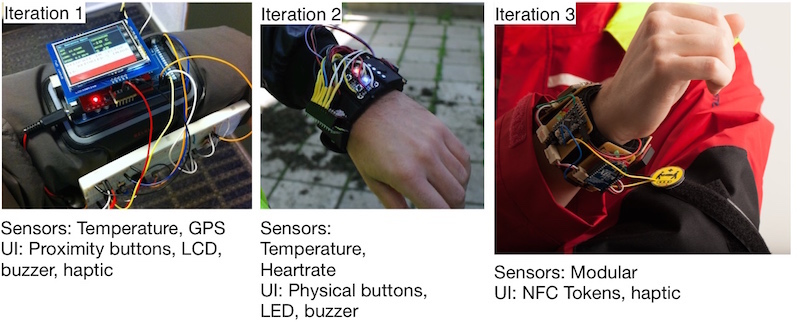
\includegraphics[width=1 
	\textwidth]{watchit_iterations} \caption{Three prototyping iterations for WATCHiT} \label{fig:watchit-prototypes} 
\end{figure}

The requirement for distraction-free user interfaces has been implemented with the design of a novel sensing-based interface grounded on previous works on mnemonic body shortcuts and body-centric interaction \autocites{Guerreiro:2008wt}{Chen:2012wk}. Those works propose to use areas of the body as shortcuts to trigger digital operations in the context to facilitate smartphone-mediated interaction with digital services. In this work body shortcuts are specialised to assist data capturing processes. Areas on work uniforms and tools (identified by RFID tags) trigger digital operation when the worker hover WATCHiT on them. Each shortcut can be pre-configured to control the activation of specific sensors and to tag the data the is being captured with contextual information. User evaluations performed during physical simulations of crisis work have shown that the interaction technique is well accepted and WATCHiT is suitable to be used during simulated crisis work.

WATCHiT has been used to capture experiential data in order to feed technology-assisted debriefings thanks to the integration with the CroMAR and Trainer app, as described in P2. A new prototype and summative evaluation for the tool is described in P6.

\emph{Relation to research questions:} The paper covers aspects of RQ1 ``\RQi''

%------PAPER 4
\section[Don't Panic: Enhancing Soft Skills for Civil Protection Workers]{Paper 4}\label{paper-4}

\emph{Title:} Don't Panic: Enhancing Soft Skills for Civil Protection Workers

\emph{Authors:} Ines Di Loreto, Simone Mora and Monica Divitini

\emph{Authors' contributions:} All the co-authors contributed to the research.~Di Loreto, first author, led the game design and coordinated the paper writing. Mora contributed to game design with his knowledge of crisis training. He also contributed to the documentation of the work in the paper.~Divitini provided~general~supervision for the research and the paper writing.

\emph{Published in:} Proceedings of the International Conference on Serious Games Development Applications (SGDA), 2012 
\begin{quote}
	\emph{Abstract:} \emph{Don't Panic} is a serious game created to enhance soft skills in the crisis management field. The game is conceived to (i) add the fun element to training about stressful situations linked to panic management and (ii) teach skills such as communication styles, team management and coordination, time management, stress management and coping strategies. In this paper we present the first paper-based version of the game and its evaluation. The paper discusses the game design motivations, the methodological reasons behind its conception, and presents a pilot study. Results show that, even in its paper version, the game is a promising tool if linked with adequate and realistic procedures. This opens methodological questions about the role of computer based serious games. 
\end{quote}

\emph{Description:} The paper investigates the use of collaborative and mobile serious games as a tool to enhance soft skills in crisis work. Serious games can complement traditional formal training by enhancing workers' communication abilities, stress management and coping skills. The fun element typical of (computer or traditional) games can act as motivation factor to engage workers in training. After presenting the state of the art of serious games for crisis training, the paper dives into the description of \emph{Don't Panic}, a board game designed by the authors. 

\emph{Don't Panic} aims at training soft skills in the management of situations where diffusion of panic might put population at risk. Each player acts as a member of a panic control team that must work together to manage panicked crowds. During a game session different potential panicking events take place in the city represented on the board. Each player assumes a unique role within a team, with special abilities that improve the team's chances, if applied wisely. The players have a limited time to calm down the situation, before the panic spreads and they lose the game. \emph{Don't Panic} has multiple aims linked to learning. The game aims at teaching communication styles useful to manage crisis events but also foster team building. It was conceived to push local vs.~global reasoning, problem dissection and making plans dividing the board into zones and adding unpredictable events during the game that can create contrasting reasoning and priorities.

The paper details game mechanics and rules. A paper prototype of \emph{Don't Panic} (Figure \ref{fig:dp-mockup}) is presented and evaluated in a pilot study with 10 crisis workers who played the game. Building on evaluation results the authors derive implications for the design of a technology-augmented version of the game (described in P5).

The addition of technology in future iterations would release the players from doing game management tasks which disrupted the game experience in the paper mockup. Moreover technology can be used to to add computer interactivity, for example by means of audio and graphic feedbacks. Secondly it can improve learning effectiveness of the game by logging players' actions to be used as traces for reflection. After a game session, the captured traces can be used to help players reflect on the actions taken during the game, and to link those actions to their real work experiences, with the goal of triggering \emph{storytelling} and therefore reflection. 

\begin{figure}
	[tbh] \centering 
	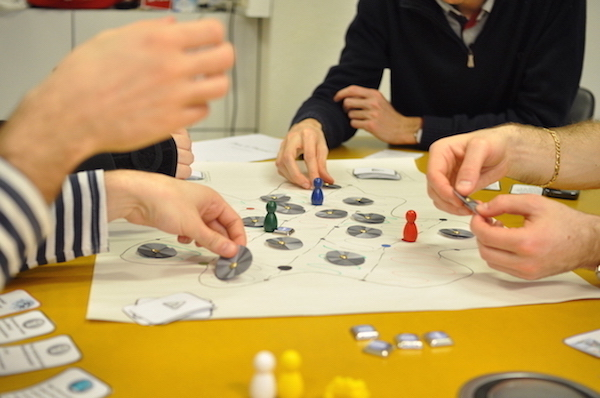
\includegraphics[width=1 
	\textwidth]{dp_mockup} \caption{Paper mockup of “Dont’ Panic!”} \label{fig:dp-mockup} 
\end{figure}

This pilot study and the derived implication for design have driven the design of an technology-enhanced version of the game presented in P5.

\emph{Relation to the research questions: } The paper contributes to the investigation of RQ2, ``\RQii''

\section[The interactive-token approach to board games]{Paper 5}\label{paper-5}

\emph{Title:} The interactive-token approach to board games

\emph{Authors:} Simone Mora, Ines Di Loreto and Monica Divitini

\emph{Authors' contributions:} Mora led the design and implementation work. He was also the~main~contributor of the paper. Di Loreto designed the board game that is used as example in the paper. Di Loreto and Mora jointly designed and attended evaluation studies.~Divitini provided~general~supervision for the research and the paper writing.

\emph{Published in:} Ready for submission 
\begin{quote}
	\emph{Abstract:} Recent advances in interactive surfaces and Tangible User Interfaces have created a new interest in digital board games, aiming at mixing the benefits of traditional board games with the interactivity of video games. Within this strand of research we propose a new approach centred on the concepts of tokens, constraints, spatial expressions and interaction events. While mainstream solutions implement game interaction using interactive surfaces, our approach relies on physical manipulation of interactive objects on conventional surfaces. We illustrate the proposed approach by describing the design and development of a game for training of emergency workers. Building on feedbacks from user evaluation and our experience with the development, we outline design opportunities and challenges of the approach. 
\end{quote}

\emph{Description:} The paper presents a novel approach to the digitalisation of board games. The approach aims at adding computer games interactivity preserving board games's traditional social and physical affordances. Rather than implementing games for interactive surfaces (e.g.~touch-screens) the approach relies on the physical manipulation of interactive objects on conventional surfaces. After reviewing state of the art technology for digital board games, the approach is presented and grounded in existing frameworks of tangible user interfaces. To facilitate implementation of the approach into the design practice of digital board games a three-steps process is presented. The process provides guidelines for designing computer-augmented game pieces and for mapping sensing-based interactions with pieces to game dynamics.

P4 introduced \emph{Don't Panic}, a serious game for enhancing soft skills for crisis workers, pointing out the role of technology as facilitator for generating engaging game experiences and for supporting post-game reflection and mapping with the real work. The approach and process presented in this paper have been used to drive a new design iteration for the game. 

In the new, technology-augmented prototype (Figure \ref{fig:dp-token}), social affordances of traditional board games, in terms of prompts for cooperation and discussion, are preserved. This is functional to the serious role of \emph{Don't Panic} as facilitator for storytelling and team building. At the same time the added computer interactivity provides a game experience which is more immersive and less disrupting compared to the paper mockup presented in P4. This allows for generating, by means of the game, a simulated work experience (management of panicking crowds) that re-create as much as possible conditions of emotional stress and decision making under time constraints, typical of real work. The prototype has been evaluated against usability with 16 players who played the game in groups of four. Results from the experiment contribute in shedding the light on opportunities and challenges offered by the presented approach.

The paper also describes the technical challenges faced by the authors during the prototyping process. A mix of software, hardware, laser-cut and 3D printing techniques have been orchestrated in order to fully implement game dynamics and produce a prototype of a game that can be played for an entire session without major disruptions. Beside allowing to implement a new version of \emph{Don't Panic} the approach proposed in the paper is a contribution in the field of TUIs which can inspire the design of new digital board games.

\begin{figure}
	[tbh] \centering 
	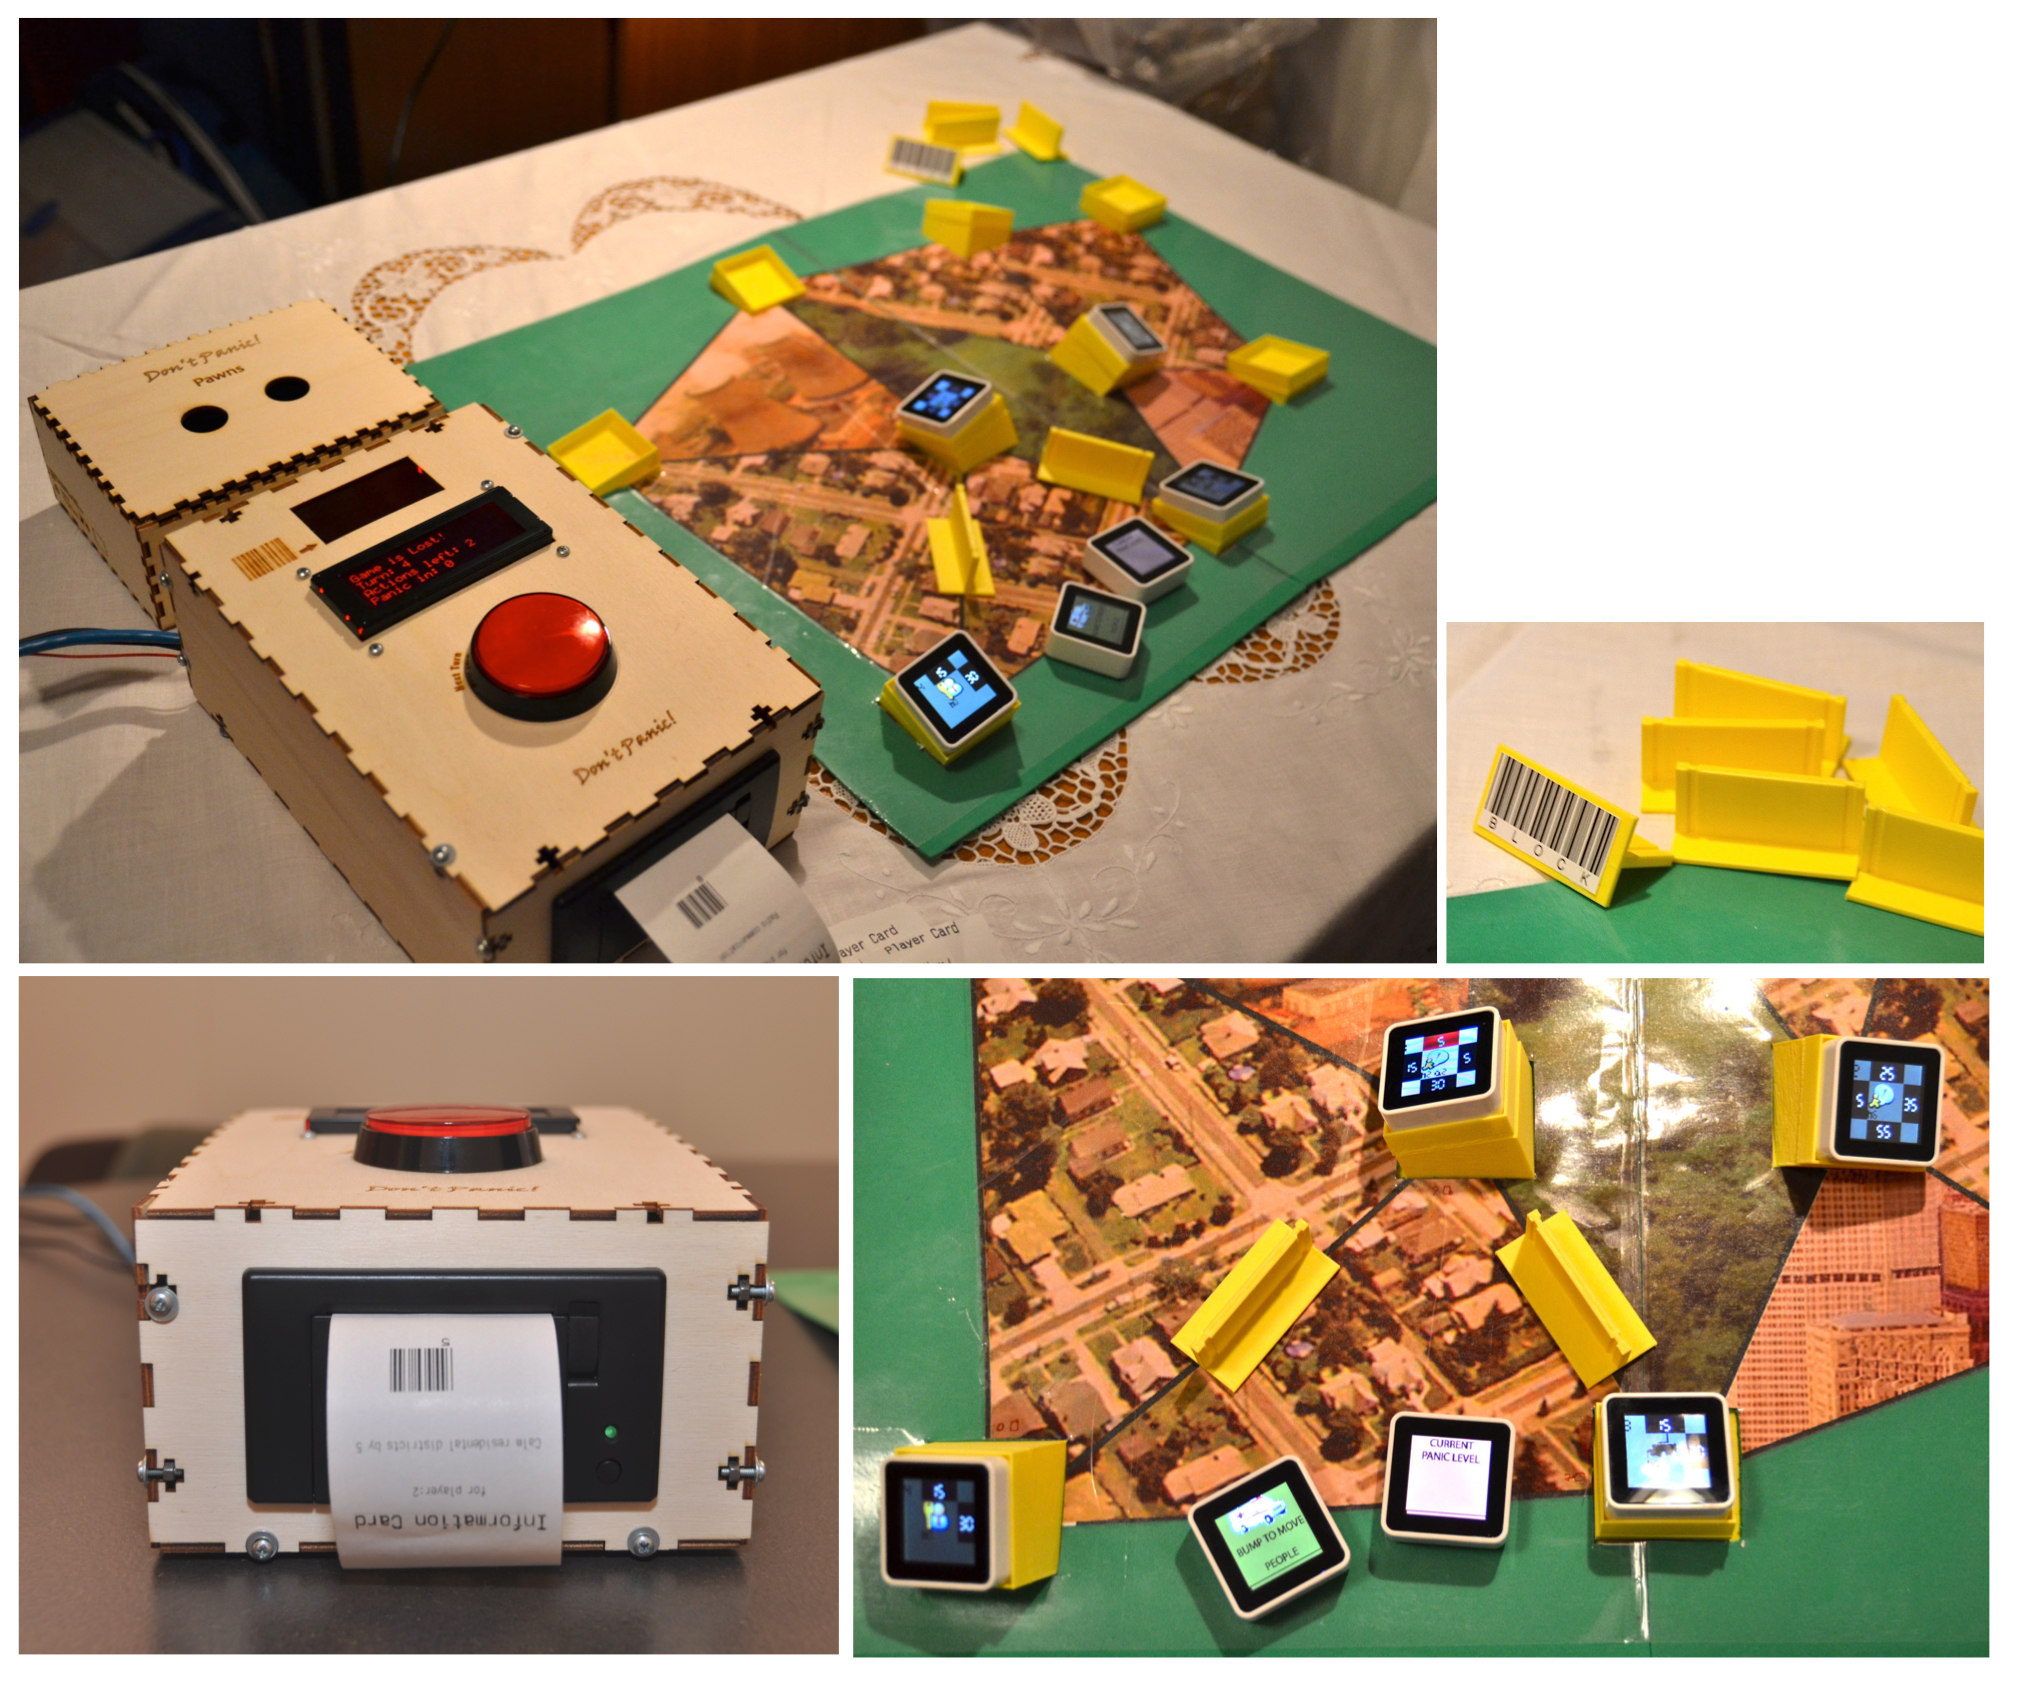
\includegraphics[width=1 
	\textwidth]{dp-multi} \caption{Technology-augmented “Don't Panic!” working prototype} \label{fig:dp-token} 
\end{figure}

\emph{Relation to the research questions: } The paper contributes to the investigation of RQ2, ``\RQii'' and RQ3, ``\RQiii''

\section[Context Becomes Content: Sensor Data for Computer-Supported Reflective Learning]{Paper 6}\label{paper-6}

\emph{Title:} Context Becomes Content: Sensor Data for Computer-Supported Reflective Learning

\emph{Authors:} Lars Müller, Monica Divitini, Simone Mora, Verónica Rivera-Pelayo and Wilhelm Stork

\emph{Authors' contributions:} Müller led the writing of the paper and contributed with one of the case studies. Mora designed the systems presented in the second case study. Mora also designed and conducted the evaluation of the system. Rivera-Pelayo contributed with state of the art about~the quantified self and to the methodological part. All the authors contributed to draw lessons learned and theoretical implications~from~the two~studies. Divitini and Stork contributed with supervision during the writing process.

\emph{Published in:} IEEE Transactions on Learning Technologies 
\begin{quote}
	\emph{Abstract:} Wearable devices and ambient sensors can monitor a growing number of aspects of daily life and work. We propose to use this context data as content for learning applications in workplace settings to enable employees to reflect on experiences from their work. Learning by reflection is essential for today's dynamic work environments, as employees have to adapt their behaviour according to their experiences. Building on research on computer-supported reflective learning as well as persuasive technology, and inspired by the Quantified Self community, we present an approach to the design of tools supporting reflective learning at work by turning context information collected through sensors into learning content. The proposed approach has been implemented and evaluated with care staff in a care home and voluntary crisis workers. In both domains, tailored wearable sensors were designed and evaluated. The evaluations show that participants learned by reflecting on their work experiences based on their recorded context. The results highlight the potential of sensors to support learning from context data itself and outline lessons learned for the design of sensor-based capturing methods for reflective learning. 
\end{quote}

\emph{Description:} This paper proposes the use of context data as content to support reflective learning in workplace settings. The approach uses technology to turn unstructured context data into learning contents. Two case studies presented in the paper demonstrate how the approach facilitates designers in mapping requirements from reflective learning theory with opportunities provided by technology, within the constraints of the specific workplace environment.

Three design decisions have to be made to turn context into content: \emph{what context} is relevant to be captured, \emph{how to capture} it and \emph{how to visualise} it to support reflection. The first two decisions were already explored drafting design challenges for data capturing tools (P3). In this paper they are further elaborated.

The paper reveals that the decision of \emph{what context} to be captured is highly situated with the work experience to be acquired. The decision is made harder by the unpredictability of outcomes typical of the reflective practice and by the need for interpretation required by the unstructured nature of context data. Yet the paper identifies three types of context that may include relevant data for reflection: \emph{task}, \emph{affective} and \emph{social}. \emph{Task context} relates directly to the work process and is therefore easy to understand. \emph{Affective context} might work as a marker to recognise relevant episodes for reflection; because if something happens during the day, it will trigger an emotional reaction that can be captured with sensors. Finally \emph{social context} is important for many collaborative work practices since the interactions with other people (colleague, customers, patients) constitute an important aspect of many experiences to reflect upon.

\emph{How to capture context} is also further elaborated in this paper. Three methods are proposed. Data can be \emph{self-reported} by the users, thus providing a subjective impression on an experience (e.g. by means of digital diaries). Data can be \emph{self-reported from third parties} in this way an external perspective is made available to the reflecting person. Finally data can be captured \emph{automatically} by sensors and applications; for example by means of stress or activity-tracking sensors.

Compared to P3 the paper adds a third design challenge connected to \emph{visualisation of context}. In order to be effective in triggering and sustaining a reflection sessions, data should be visualised from multiple perspective. Discrepancies among different view of the same experience should be outlined as reflection triggers. The social (comparing data over multiple users), spatial (the location data were captured) and historical perspectives (evolution of data samples over time) are considered as effective for reflection. The CroMAR app (P1) and Trainer app (P2) were designed to visualise data according with one or more of those perspectives.

The three design dimensions are functional to build technology tools that implement the stages of the CSRL cycle (Chapter \ref{csrl}). While what context and how to capture it pertains designing of technology to support the \emph{plan and do work} stage of the model, \emph{how to visualise data} provides support for the subsequent stages of \emph{initiate reflection} and \emph{conduct reflection session}. To motivate the user in the data collection process methods borrowed from persuasive technology and quantified self are presented.

The paper further presents two case studies and their evaluation. One of the cases show the use of WATCHiT (P3) and Trainer (P2) to support reflection on the implementation of protocols (e.g.~medical procedures) by workers in the field, immediately after the procedure is performed. The system promotes a quick reflection session with easy triggers that can be done by the worker herself or collaboratively by a team. The second case study is an application designed to support carers in dementia care homes by reflecting on their daily interaction with residents and colleagues. Both case studies have target users -carers and crisis workers-, that work in highly dynamic environments and therefore benefit the most from on-the-job, reflective training.

Field evaluations for two case studies show that participants were able to learn from the visualised context. Yet, it is confirmed that learning goals and expected outcomes are difficult to be defined a priori. It is also considered important to provide an option to record reflection outcomes, so that the gained insight can be user later (and might trigger new reflection cycles). Capturing tools should be easy to adapt, in order to allow the users to deal with the unpredictability of relevance of the captured context. This choice has been implemented in WATCHiT (P3) by means of physical sensor modules.

\emph{Relation to the research questions: } The paper dresses RQ1 ``\RQi'' and RQ2, ``\RQii''

\section[A Unified Architecture for Supporting Direct Tag-Based and Indirect Network-Based Resource Discovery]{Paper 7}\label{paper-7}

\emph{Title:} A Unified Architecture for Supporting Direct Tag-Based and Indirect Network-Based Resource Discovery

\emph{Authors:} Simone Mora and Babak Farshchian

\emph{Authors' contribution:} Mora conducted the design work and wrote the paper. Farshchian provided feedbacks throughout both the design and writing processes.

\emph{Published in:} Proceedings of the European Conference on Ambient Intelligence (AMI), 2010 
\begin{quote}
	\emph{Abstract:} Discovering and integrating ambient computational resources is a central topic in AmI. There are two major existing approaches: indirect network-based resource selection and direct tag-based resource identification. We motivate the need to integrate the two approaches through a scenario. We then present an architecture for a pluggable discovery system called UbiDisco. We demonstrate how UbiDisco implements a seamless integration of the two approaches at user interaction level through a framework for implementing discovery actions. 
\end{quote}

\emph{Description:} This paper presents a modular approach to software components for service discovery that blends the benefits of direct tag-based and indirect network-based discovery. The approach has been implemented in a middleware, called \emph{UbiDisco}, that allows for discovery and customisation of computational resources and support data exchange between heterogeneous systems. \emph{UbiDisco} is both a middleware and a collection of user interfaces for service discovery.

The work constitute a foundation of the rapid prototyping approach pursued in this PhD. As demonstrated in P2 and P6 the CSRL cycle is supported by a set of diverse technologies spanning from wearable and physical computers to apps for tablets and smartphones. Enable workers to easily link those tools in order to allow data exchange is critical to build custom, scenario-specific ecologies of tools to support the different stages of the reflection cycle. Integrating different apps is technically complex since it involves serialisation of data, configuration of wireless networks and interaction of back-end services such as databases. From the perspective of the user it involves filling in configuration details. This activity might be very complex on mobile and wearable tools.

UbiDisco hinders the user from the complexity of configuring technical details by means of \emph{discovery actions}. The user can link two systems by reading a barcode or RFID tag which identifies the device/service and provide technical details for the configuration of the link. For example CroMAR running on a iPad can be linked to WATCHiT, by reading a barcode printed on the device hardware. In this way WATCHiT and CroMAR network addresses and protocols in use are exchanged between the two systems. WATCHiT becomes a data provider for CroMAR until a new \emph{discovery action} links WATCHiT to a new system (e.g.~another instance of CroMAR or Trainer).

\emph{Relation to the research questions: } The paper contributes to RQ3, ``\RQiii'' 
